\documentclass[border=4pt]{standalone}
\usepackage{tikz}
\usepackage{pgfplots}
\pgfplotsset{compat=1.18}
\usetikzlibrary{shapes.geometric,arrows.meta,positioning,calc,fit,decorations.pathreplacing,backgrounds}
\definecolor{boxblue}{RGB}{225,238,252}
\definecolor{boxgreen}{RGB}{225,247,231}
\definecolor{boxorange}{RGB}{253,236,216}
\definecolor{boxgray}{RGB}{237,237,237}
\definecolor{boxred}{RGB}{253,226,226}
\begin{document}
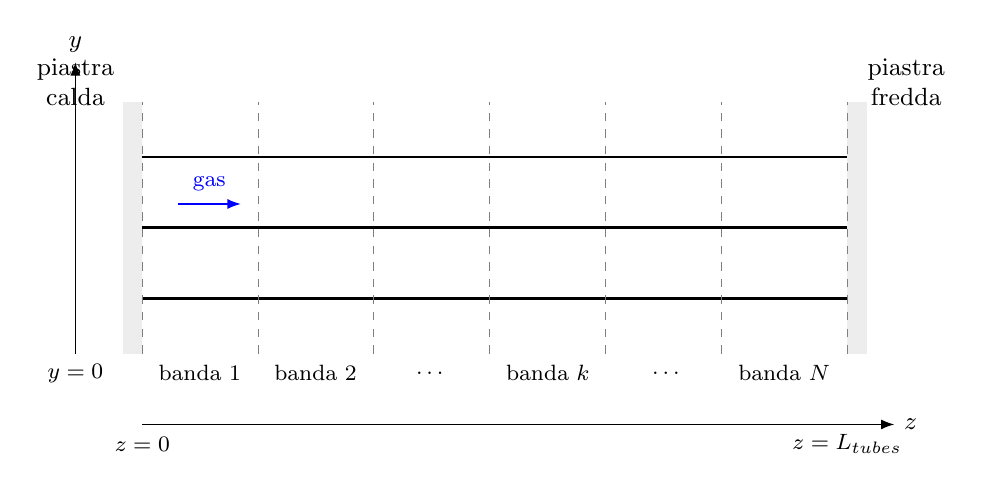
\begin{tikzpicture}[scale=1.0]
% Tubesheet hot (left) and cold (right)
\fill[boxgray] (0,-1.6) rectangle (0.25,1.6);
\fill[boxgray] (9.2,-1.6) rectangle (9.45,1.6);
\node[font=\small,align=center] at (-0.6,1.85) {piastra\\calda};
\node[font=\small,align=center] at (9.95,1.85) {piastra\\fredda};

% Tubes (3 lines to represent bundle)
\foreach \y in {-0.9,0,0.9}{
  \draw[thick] (0.25,\y) -- (9.2,\y);
}

% Band divisions
\foreach \x in {0.25,1.72,3.19,4.66,6.13,7.6,9.2}{
  \draw[dashed,gray] (\x,-1.6) -- (\x,1.6);
}
\node[font=\footnotesize] at (0.98,-1.85) {banda 1};
\node[font=\footnotesize] at (2.45,-1.85) {banda 2};
\node[font=\footnotesize] at (3.9,-1.85) {$\ldots$};
\node[font=\footnotesize] at (5.4,-1.85) {banda $k$};
\node[font=\footnotesize] at (6.9,-1.85) {$\ldots$};
\node[font=\footnotesize] at (8.4,-1.85) {banda $N$};

% axes
\draw[-{Latex}] (0.25,-2.5) -- (9.8,-2.5) node[right,font=\small] {$z$};
\draw[-{Latex}] (-0.6,-1.6) -- (-0.6,2.1) node[above,font=\small] {$y$};
\node[font=\footnotesize] at (-0.6,-1.85) {$y=0$};
\node[font=\footnotesize] at (0.25,-2.75) {$z=0$};
\node[font=\footnotesize] at (9.2,-2.75) {$z=L_{tubes}$};

% gas flow arrow inside tube
\draw[-{Latex},blue] (0.7,0.3) -- (1.5,0.3);
\node[font=\footnotesize,blue] at (1.1,0.55) {gas};
\end{tikzpicture}
\end{document}
